\documentclass[main.tex]{subfiles}

% Load any packages needed for this document
\begin{document}
%-------------------------------------------------------------------------------------------%
\newpage
\section{Regression Diagnostics with \texttt{R} }
% http://www.statmethods.net/stats/rdiagnostics.html

An excellent review of regression diagnostics is provided in John Fox's aptly named \textit{Overview of Regression Diagnostics}. Dr. Fox's car package provides advanced utilities for regression modeling.

\begin{verbatim}
(1) Fox, John. (1991). Regression Diagnostics: An Introduction. Sage Publications.
\end{verbatim}

\begin{framed}
\begin{verbatim}
# Assume that we are fitting a multiple linear regression
# on the MTCARS data
library(car)
fit <- lm(mpg~disp+hp+wt+drat, data=mtcars)

\end{verbatim}
\end{framed}


\subsection{Outliers}

Assessment of Outliers can be carried out using the \texttt{outlierTest} function.

\begin{framed}
\begin{verbatim}
outlierTest(fit) # Bonferonni p-value for most extreme obs
qqPlot(fit, main="QQ Plot") #qq plot for studentized resid 
leveragePlots(fit) # leverage plots
\end{verbatim}
\end{framed}
\subsection{Added Variable Plots}
\begin{framed}
\begin{verbatim}
# added variable plots 
av.Plots(fit)
\end{verbatim}
\end{framed}

\subsection{Non-constant Error Variance}
\begin{framed}
\begin{verbatim}

# Evaluate homoscedasticity
# non-constant error variance test
ncvTest(FitMod)
# plot studentized residuals vs. fitted values 
spreadLevelPlot(FitMod)
\end{verbatim}
\end{framed}

\begin{verbatim}
> ncvTest(FitMod)
Non-constant Variance Score Test 
Variance formula: ~ fitted.values 
Chisquare = 3.330027    Df = 1     p = 0.06802577 
\end{verbatim}

%mtcarsSpreadLevel Plot here

\begin{figure}[h!]
\centering
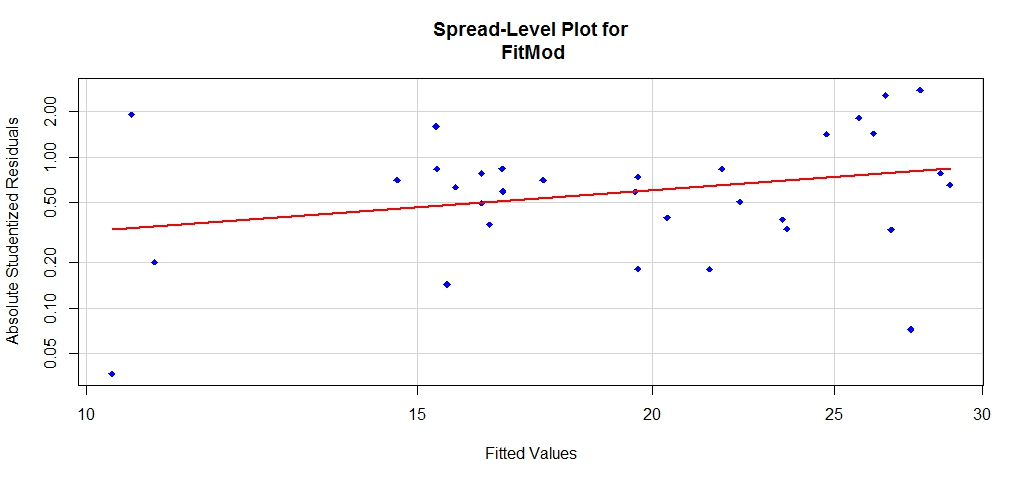
\includegraphics[width=0.7\linewidth]{./mtcarsSpreadLevelPlot}
\label{mtcarsSpreadLevelPlot}
\end{figure}


\begin{verbatim}
Suggested power transformation:  0.08866484 
\end{verbatim}

\subsection{Influential Observations}
\begin{framed}
\begin{verbatim}
# Influential Observations

# Cook's D plot
# identify D values > 4/(n-k-1) 
cutoff <- 4/((nrow(mtcars)-length(fit$coefficients)-2)) 
plot(fit, which=4, cook.levels=cutoff)
# Influence Plot 
influencePlot(fit,	 id.method="identify", main="Influence Plot", sub="Circle size is proportial to Cook's Distance" )
\end{verbatim}
\end{framed}
%-------------------------------------------------------------- %
\newpage
\section{Diagnostic Plots for Linear Models with \texttt{R}}
Plot Diagnostics for an \texttt{lm} Object

\subsection{Description}

Six plots (selectable by \texttt{which}) are currently available: 
\begin{enumerate}
\item a plot of residuals against fitted values, 
\item a Scale-Location plot of \textit{sqrt(| residuals |}) against fitted values, 
\item a Normal Q-Q plot, 
\item a plot of Cook's distances versus row labels, 
\item a plot of residuals against leverages, 
\item a plot of Cook's distances against leverage/(1-leverage).
\end{enumerate} By default, the first three and 5 are provided.
\newpage
%http://stats.stackexchange.com/questions/58141/interpreting-plot-lm
 I explained the assumption of homoscedasticity and the plots that can help you assess it (including scale-location plots [2]) on CV here: What does having constant variance in a linear regression model mean? I have discussed qq-plots [3] on CV here: QQ plot does not match histogram. So, what's left is primarily just understanding [5], the residual-leverage plot.

To understand this, we need to understand three things:

\begin{itemize}
\item leverage,
\item standardized residuals, and
\item Cook's distance.
\end{itemize}
%Move next bit to "Leverarge"
\subsubsection{Leverage}
To understand leverage, recognize that \textit{Ordinary Least Squares} regression fits a line that will pass through the centre of your data, ($\bar{x}, \bar{y}$). The line can be shallowly or steeply sloped, but it will pivot around that point like a lever on a fulcrum. We can take this analogy fairly literally: because OLS seeks to minimize the vertical distances between the data and the line, the data points that are further out towards the extremes of X will push / pull harder on the lever (i.e., the regression line); they have more leverage. One result of this could be that the results you get are driven by a few data points; that's what this plot is intended to help you determine.

% Standardization
Another result of the fact that points further out on X have more leverage is that they tend to be closer to the regression line (or more accurately: the regression line is fit so as to be closer to them) than points that are near $\bar{x}$. In other words, the residual standard deviation can differ at different points on X (even if the error standard deviation is constant). To correct for this, residuals are often standardized so that they have constant variance (assuming the underlying data generating process is homoscedastic, of course).

% Cook's Distance
One way to think about whether or not the results you have were driven by a given data point is to calculate how far the predicted values for your data would move if your model were fit without the data point in question. This calculated total distance is called \textbf{Cook's distance}. Fortunately, you don't have to rerun your regression model N times to find out how far the predicted values will move, Cook's D is a function of the leverage and standardized residual associated with each data point.

With these facts in mind, consider the plots associated with four different situations:
\begin{enumerate}
\item a dataset where everything is fine
\item a dataset with a high-leverage, but low-standardized residual point
\item a dataset with a low-leverage, but high-standardized residual point
\item a dataset with a high-leverage, high-standardized residual point
\end{enumerate}
\newpage
\subsection{Diagnostic Plots for LMs}
%-------------------------------------------------------------------------------------------%
\begin{itemize}
\item
The \textbf{Scale-Location} plot, also called ‘Spread-Location’ (or ‘S-L’ plot), takes the square root of the absolute residuals in order to diminish skewness (sqrt($|E|)$) is much less skewed than $| E |$ for Gaussian zero-mean E).

\item
The \textbf{Residual-Leverage} plot shows contours of equal Cook's distance, for values of \texttt{cook.levels} (by default 0.5 and 1) and omits cases with leverage one with a warning. If the leverages are constant (as is typically the case in a balanced aov situation) the plot uses factor level combinations instead of the leverages for the x-axis. \\
\textit{(The factor levels are ordered by mean fitted value.)}
\end{itemize}
\begin{framed}
\begin{verbatim}
plot(lm(mpg~wt+cyl),which=c(1),pch=18,col="red")
plot(lm(mpg~wt+cyl),which=c(2),pch=18,col="red")
plot(lm(mpg~wt+cyl),which=c(3),pch=18,col="red")
plot(lm(mpg~wt+cyl),which=c(4),pch=18,col="red")
plot(lm(mpg~wt+cyl),which=c(5),pch=18,col="red")
plot(lm(mpg~wt+cyl),which=c(6),pch=18,col="red")
\end{verbatim}
\end{framed}

\begin{figure}[h!]
\centering
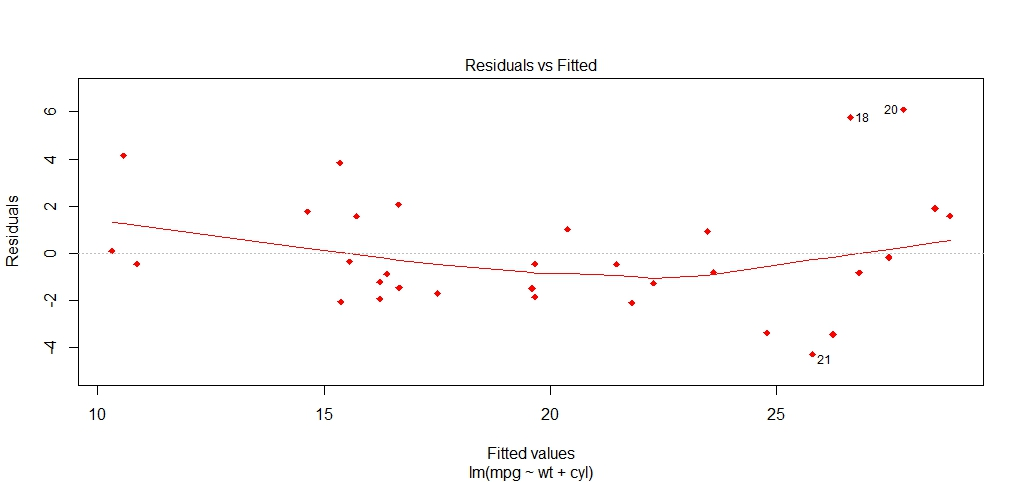
\includegraphics[width=0.9\linewidth]{./mtcarsDiagPlot1}

\label{mtcarsDiagPlot1}
\end{figure}

\newpage
\begin{figure}[h!]
\centering
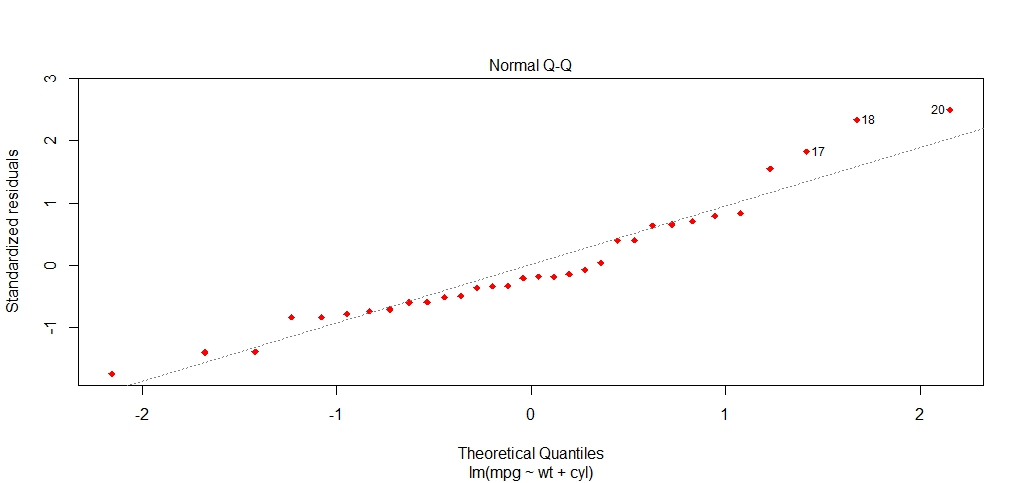
\includegraphics[width=0.9\linewidth]{./mtcarsDiagPlot2}

\label{mtcarsDiagPlot2}
\end{figure}

\subsubsection{Plot 3 : Normal Probability Plot}
This plot is used to assess the validity of the normality of the residuals.
\begin{figure}[h!]
\centering
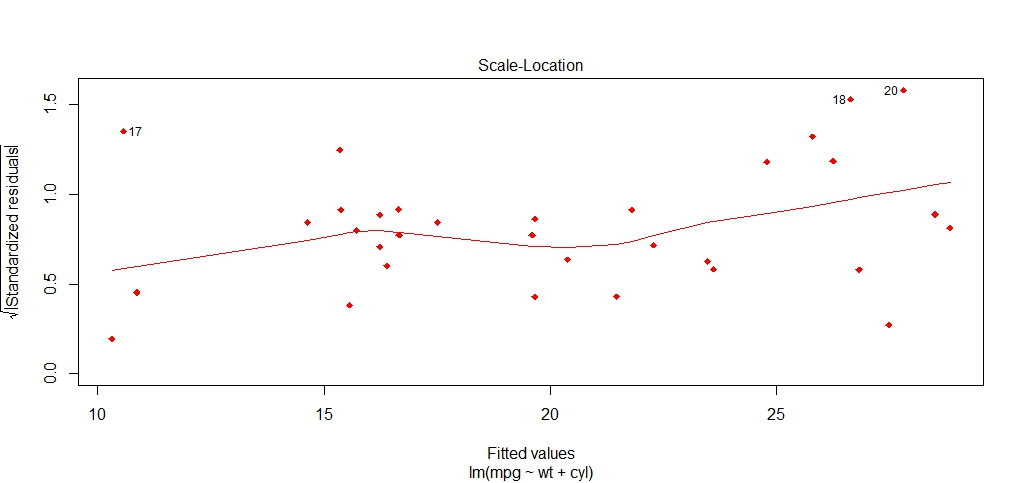
\includegraphics[width=0.9\linewidth]{./mtcarsDiagPlot3}

\label{mtcarsDiagPlot3}
\end{figure}

\newpage
\subsubsection{Plot 5 :  Cook's Distance}
\begin{figure}[h!]
\centering
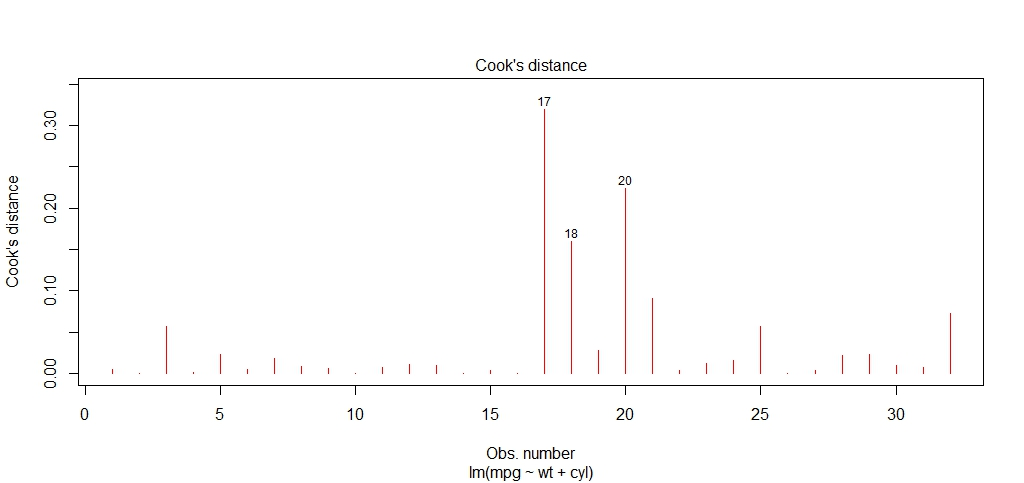
\includegraphics[width=0.9\linewidth]{./mtcarsDiagPlot4}

\label{mtcarsDiagPlot4}
\end{figure}


\begin{figure}[h!]
\centering
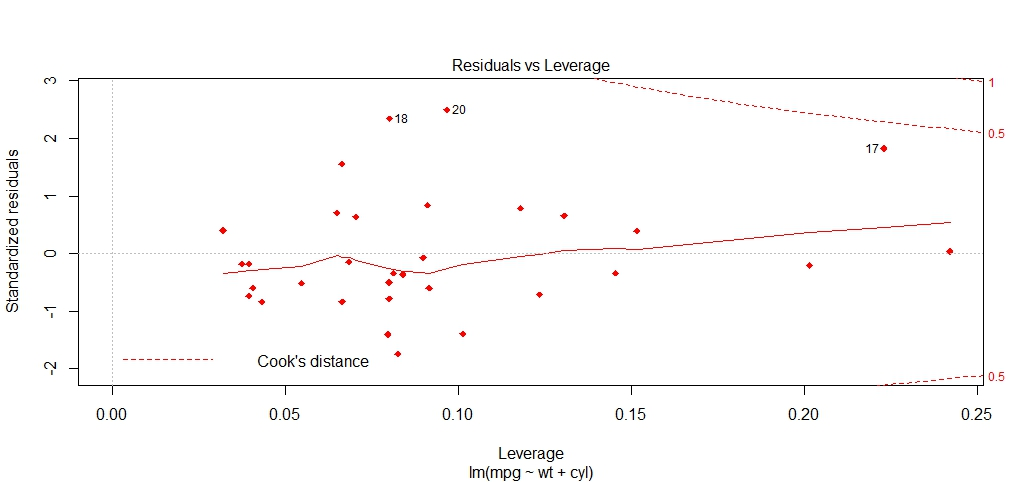
\includegraphics[width=0.9\linewidth]{./mtcarsDiagPlot5}

\label{mtcarsDiagPlot5}
\end{figure}


\subsubsection{Plot 6 :  Cook's Distance vs Leverage}
\begin{figure}[h!]
\centering
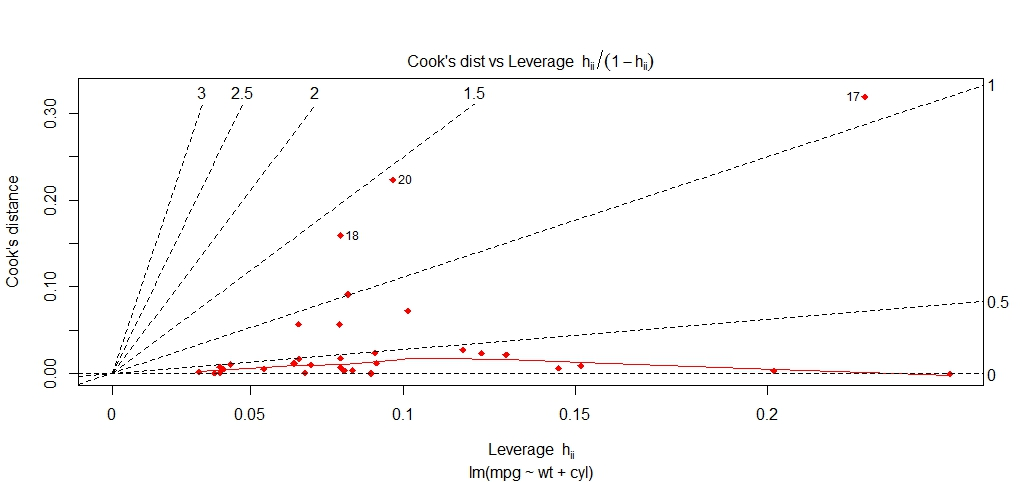
\includegraphics[width=0.9\linewidth]{./mtcarsDiagPlot6}

\label{mtcarsDiagPlot6}
\end{figure}


\begin{framed}
\begin{verbatim}
par(mfrow=c(4,1))
plot(fittedmodel)
par(opar)
\end{verbatim}
\end{framed}

% http://www.columbia.edu/~cjd11/charles_dimaggio/DIRE/resources/R/rFunctionsList.pdf

\end{document}
